\documentclass{article}
\usepackage{amsmath}
\usepackage{amssymb}
\usepackage[spanish]{babel}
\usepackage{color}
\usepackage{colortbl}
\usepackage{float}
\usepackage[T1]{fontenc}
\usepackage[rmargin=3cm,lmargin=3cm,tmargin=3cm,bmargin=4cm]{geometry}
\usepackage[utf8]{inputenc}
\usepackage{latexsym}
\usepackage{multirow}
\usepackage[spanish]{syllogism}
\usepackage{tikz}
\usepackage{tikz-qtree}
\usepackage{upgreek}

\clubpenalty=10000
\widowpenalty=10000

\begin{document}

\title{Ayudantía Unidad 1: Lógica (parte 2)}
\author{Teoría de la Computación 2-2025}
\date{}

\maketitle

\section{Lógica proposicional: Resolución}
Utilice el método de resolución para determinar si los siguientes resultados son
correctos:

\subsection{Ejemplo 1}
Queremos verificar si $\Sigma \vDash \upvarphi$ para:

$$\Sigma = \{A \rightarrow (B \vee C),\ A,\ \neg B\}$$
$$\upvarphi = C$$

\textbf{Paso 1:} escribir $\Sigma \vDash \{\neg \upvarphi\}$ en FNC (es decir,
como una conjunción de cláusulas):
\begin{itemize}
  \item{\makebox[6cm][l]{$A \rightarrow (B \vee C) \Leftrightarrow \underbrace{\neg A \vee (B \vee C)}_{C_{1}}$}
        (premisa 1)}

  \item{\makebox[6cm][l]{$\underbrace{A}_{C_{2}}$} (premisa 2)}
  \item{\makebox[6cm][l]{$\underbrace{\neg B}_{C_{3}}$} (premisa 3)}
  \item{\makebox[6cm][l]{$\underbrace{\neg C}_{C_{4}}$} (negación de la
        consecuencia)}
\end{itemize}

\textbf{Paso 2:} aplicar la regla de resolución buscando encontrar una
contradicción.

\begin{figure}[H]
  \centering
  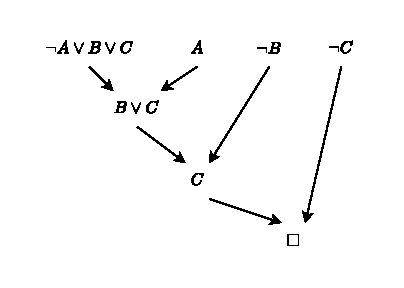
\includegraphics[width=.45\textwidth]{images/resolucion_01.pdf}
\end{figure}

Por lo tanto, logramos demostrar que:
$$\{A \rightarrow (B \vee C),\ A,\ \neg B\} \vDash C$$

\newpage

\subsection{Ejemplo 2}
Si consumo frutas, entonces tengo energía. Puedo consumir frutas o comida
chatarra. Si consumo comida chatarra, entonces me enfermo. Por lo tanto, tengo
energía o estoy enfermo.

\textbf{Paso 0:} formalizaremos el enunciado a través de las siguientes
variables:
\begin{itemize}
  \item $p$: consumo frutas
  \item $q$: tengo energía
  \item $r$: consumo comida chatarra
  \item $s$: me enfermo
\end{itemize}

Así, podemos expresar el conjunto de premisas $\Sigma$ y la conclusión lógica
$\upvarphi$ como:
$$\Sigma = \{p \rightarrow q,\ p \vee r,\ r \rightarrow s\}$$
$$\upvarphi = q \vee s$$

\textbf{Paso 1:}
\begin{itemize}
  \item{\makebox[6cm][l]{$p \rightarrow q \Leftrightarrow \underbrace{\neg p \vee q}_{C_{1}}$}
        (premisa 1)}
  \item{\makebox[6cm][l]{$\underbrace{p \vee r}_{C_{2}}$} (premisa 2)}
  \item{\makebox[6cm][l]{$r \rightarrow s \Leftrightarrow \underbrace{\neg r \vee s}_{C_{3}}$}
        (premisa 3)}
  \item{\makebox[6cm][l]{$\neg(q \vee s) \Leftrightarrow \underbrace{\neg q}_{C_{4}} \land \underbrace{\neg s}_{C_{5}}$}
        (negación de la consecuencia)}
\end{itemize}

\textbf{Paso 2:}
\begin{figure}[H]
  \centering
  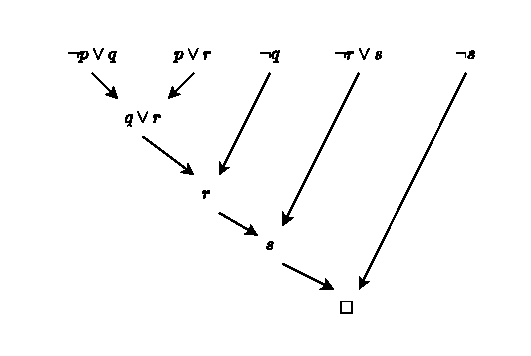
\includegraphics[width=.6\textwidth]{images/resolucion_02.pdf}
\end{figure}







\subsection{Ejemplo 3}

Queremos verificar si $\Sigma \vDash p \rightarrow (\neg r \land \neg s)$
para el conjunto de premisas:

$$\Sigma = \{p \rightarrow \neg q,\ \neg q \rightarrow (\neg r \land s), \ t,\ t\rightarrow q\}$$



\section{Lógica de primer orden: formas normales}

\begin{enumerate}
  \item Obtenga la forma normal prenexa de:
  $$\neg[\forall x \exists y\ M(x, y, z) \rightarrow \exists x (\neg \forall y\ G(y, w) \rightarrow H(x))]$$

  \item Obtenga la forma normal de Skolem de:
  $$\neg \forall x \exists r \forall y \exists z \exists w [(\neg S(x, z) \land P(b, y)) \vee (\neg P(x, z) \land S(w, r))]$$


\end{enumerate}


\end{document}
